\subsection{Device screens}\label{subsec:device-screens}
\textbf{Devices screen} (Figure \ref{fig:devices}) shows itself after a user clicks on My Devices button in \textbf{Profile screen}.
This screen contains a list of registered Dronetag devices.
In addition, here a user can add a new device which bought via Add button.

\textbf{Device screen} (Figure \ref{fig:device_detail}) contains all information about the given device including those which broadcasts in real time.
A user can choose the default device or set the device by his own needs here.

\textbf{Device registration screen} (Figure \ref{fig:device_registration}) is for registration of new device that the user bought.
It contains two text fields for typing a serial number and optional name for better identification.
After successful registration, the user is redirected to \textbf{Devices screen}.


\begin{figure}
    \centering
    \begin{minipage}{.45\textwidth}
        \centering
        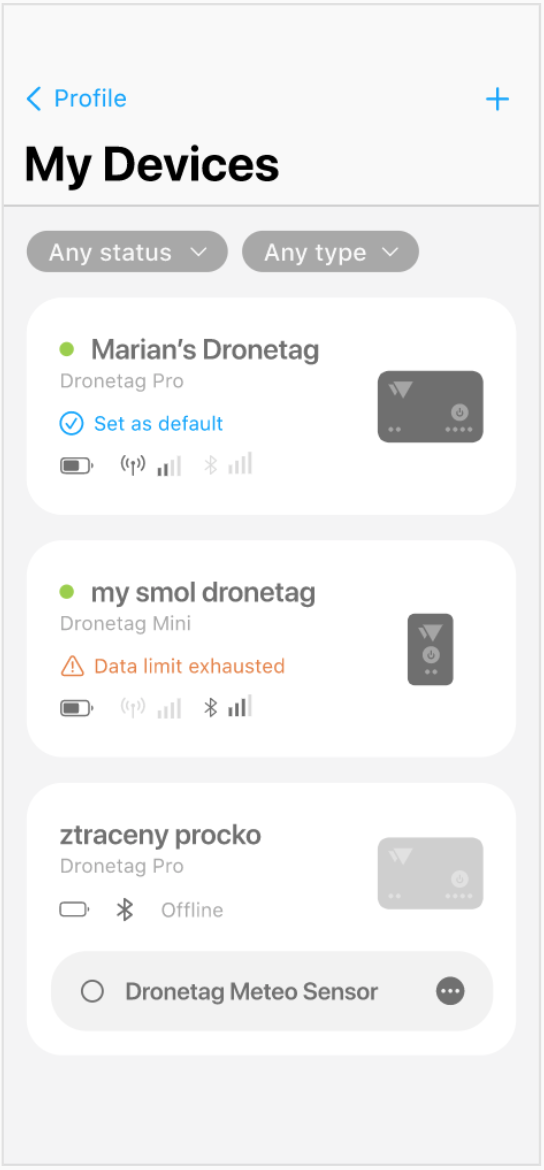
\includegraphics[width=.7\linewidth]{assets/user_interface_design/device/devices.png}
        \caption{[A20] Devices}
        \label{fig:devices}
    \end{minipage}%
    \hspace{.05\linewidth}
    \begin{minipage}{.45\textwidth}
        \centering
        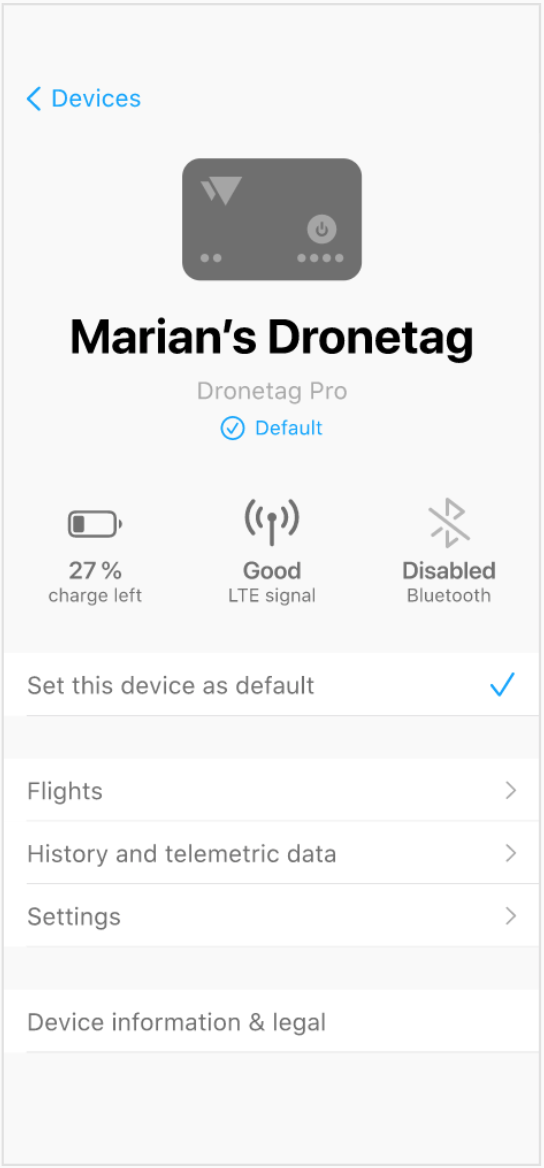
\includegraphics[width=.7\linewidth]{assets/user_interface_design/device/device_detail.png}
        \caption{[A21] Device Detail}
        \label{fig:device_detail}
    \end{minipage}
    \label{fig:device_all}
\end{figure}

\begin{figure}
    \centering
    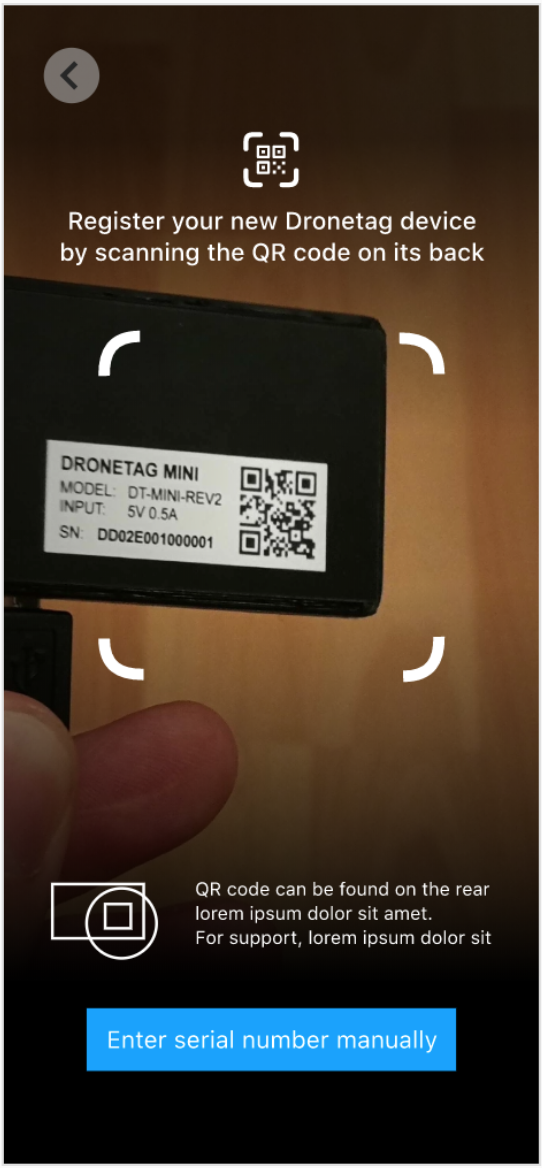
\includegraphics[width=.3\linewidth]{assets/user_interface_design/device/device_registration.png}
    \caption{[A22] Device Registration}
    \label{fig:device_registration}
\end{figure}
